% =================================================================
% Journal club: MetaScale-CO (proposal nháp, nhắm ICML 2027)
% MSO Lab, BKAI. Flow đã duyệt: FLOW.md
% Build: latexmk -pdf -interaction=nonstopmode -halt-on-error main.tex
% =================================================================
\documentclass[t, aspectratio=169]{beamer}
\usepackage[utf8]{vietnam}
\usepackage{amsthm,amsmath,amssymb}
\usepackage{lmodern}

\def\slideContentLeftMargin{0.5cm}
\def\slideContentRightMargin{1cm}
\def\hustHeaderHeight{1.5cm}
\def\slideContentBotMargin{3.5cm}

\usepackage[blue, 169]{beamerthemeHUST}
\setbeamertemplate{footline}{\vspace{1cm}}

\renewcommand{\drawHustPageNum}{%
	\ifHustShowPageNum
	\begin{tikzpicture}[remember picture, overlay]
		\node[anchor=south east, xshift=-0.35cm, yshift=0.1cm] at (current page.south east)
		{\color{hustprimary} \bfseries \small \insertframenumber};
	\end{tikzpicture}%
	\fi
}

\usepackage{pgfplots}
\pgfplotsset{compat=1.18}
\usetikzlibrary{arrows.meta,positioning,calc,shapes.geometric,decorations.pathreplacing,backgrounds,fit}
\usepackage{booktabs,multirow,colortbl,array}
\usepackage{pifont}
\usepackage[linesnumbered,ruled,vlined]{algorithm2e}
\usepackage[most]{tcolorbox}

\definecolor{cin}{HTML}{2E86C1}
\definecolor{chid}{HTML}{F39C12}
\definecolor{cout}{HTML}{27AE60}
\definecolor{cred}{HTML}{CE1628}
\definecolor{cgray}{HTML}{7F8C8D}

\tikzset{
	box/.style={rectangle,rounded corners=3pt,draw=hustprimary,thick,fill=hustprimary!8,align=center,inner sep=4pt,font=\small},
	rbox/.style={box,draw=cred,fill=cred!8},
	gbox/.style={box,draw=cout,fill=cout!10},
	obox/.style={box,draw=chid,fill=chid!12},
	arr/.style={-{Stealth[length=2mm]},thick},
	barr/.style={-{Stealth[length=2mm]},thick,cred,dashed},
}

\newcommand{\keymsg}[1]{\par\vspace{0.12cm}\noindent\makebox[\linewidth][c]{\colorbox{hustprimary!10}{\parbox{0.92\linewidth}{\centering\small\color{hustprimary}\textbf{#1}}}}\par}
\newcommand{\slidesource}[1]{\par\nointerlineskip\vbox to0pt{\hbox{%
    \begin{tikzpicture}[remember picture,overlay]
    \node[anchor=south east,xshift=-0.5cm,yshift=0.65cm,font=\scriptsize,text=black!65]
    at (current page.south east) {Nguồn: #1};
    \end{tikzpicture}}\vss}}
\newcommand{\best}[1]{\textbf{#1}}

% --- Công thức đóng khung: \eqb{số Eq.}{công thức} ---
\tcbset{eqstyle/.style={enhanced,colback=hustprimary!5,colframe=hustprimary,boxrule=0.7pt,arc=2pt,
		left=4pt,right=4pt,top=3pt,bottom=1pt,before skip=5pt,after skip=2pt,
		attach boxed title to top right={xshift=-3mm,yshift=-2.2mm},
		boxed title style={colback=hustprimary,colframe=hustprimary,boxrule=0pt,arc=1pt,left=2pt,right=2pt,top=0pt,bottom=0pt},
		fonttitle=\tiny\bfseries,coltitle=white}}
\newcommand{\eqb}[3][]{%
	\begin{tcolorbox}[eqstyle,title={Eq.~#2}]
		\centerline{$\displaystyle #3$}%
		\if\relax\detokenize{#1}\relax\else
		\par\vspace{1pt}{\scriptsize\color{black!80}\textbf{\color{hustprimary}Nghĩa:} #1\par}\fi
	\end{tcolorbox}}
% Hộp ghi chú nhỏ
\newcommand{\smallnote}[1]{{\footnotesize\color{black!70}#1}}
\newcommand{\minhhoa}{{\scriptsize\itshape\color{cgray}(minh hoạ, không phải số liệu thật)}}

\renewcommand{\titlePageTitleX}{-0.5cm}
\renewcommand{\titlePageTitleY}{-0.5cm}
\renewcommand{\hustTitleAlign}{\alignLeft}
\renewcommand{\hustSubtitleAlign}{\alignLeft}
\renewcommand{\hustAuthorAlign}{\alignLeft}
\renewcommand{\hustInstAlign}{\alignLeft}

\title{MetaScale-CO}
\subtitle{Học cách tiêu test-time compute cho tối ưu tổ hợp}
\author{\texorpdfstring{Le Viet Anh - 202516698}{Le Viet Anh - 202516698}}
\institute{}

\begin{document}

	\hustintropage{}
	\husttitlepage

	\begin{frame}{Nội dung trình bày}
		\vspace*{-6mm}\small\tableofcontents[hideallsubsections]
	\end{frame}

	\resetPageCount
	\showPageNumber
	\useStyleHustFull
	\useThinBar

	% =================================================================
	\section{Khái niệm nền}

	\begin{frame}{Khái niệm nền (1/2): bài toán và solver}
		\centering\footnotesize
		\renewcommand{\arraystretch}{1.12}
		\begin{tabular}{@{}>{\raggedright\arraybackslash\leavevmode\color{hustprimary}\bfseries}p{0.22\textwidth}>{\raggedright\arraybackslash}p{0.42\textwidth}>{\raggedright\arraybackslash}p{0.28\textwidth}@{}}
			\toprule
			\color{black}Thuật ngữ & \textbf{Định nghĩa ngắn} & \textbf{Ví dụ} \\
			\midrule
			Tối ưu tổ hợp (CO) & chọn phương án tốt nhất trong tập hữu hạn cực lớn & thứ tự giao 20 đơn hàng \\
			TSP & qua mọi thành phố đúng 1 lần rồi về, đường ngắn nhất & TSP-100: $99!/2$ chu trình \\
			MIS & chọn nhiều đỉnh nhất, không 2 đỉnh nào kề nhau & mời khách không ai ghét nhau \\
			Neural CO solver & mạng neural học từ nhiều instance để sinh lời giải & DIFUSCO, GenSCO \\
			Diffusion model & sinh lời giải bằng khử nhiễu từng bước & ảnh mờ được làm nét dần \\
			Test-time compute & tính thêm \emph{lúc dùng} model, không phải lúc train & làm bài xong rồi soát lại \\
			Optimality gap & $100\cdot(f-f^{\mathrm{ref}})/f^{\mathrm{ref}}$ (\%) & $7.85$ vs.\ $7.76$ $\Rightarrow1.16\%$ \\
			\bottomrule
		\end{tabular}
	\end{frame}

	\begin{frame}{Khái niệm nền (2/2): ra quyết định về compute}
		\centering\footnotesize
		\renewcommand{\arraystretch}{1.12}
		\begin{tabular}{@{}>{\raggedright\arraybackslash\leavevmode\color{hustprimary}\bfseries}p{0.22\textwidth}>{\raggedright\arraybackslash}p{0.42\textwidth}>{\raggedright\arraybackslash}p{0.28\textwidth}@{}}
			\toprule
			\color{black}Thuật ngữ & \textbf{Định nghĩa ngắn} & \textbf{Ví dụ} \\
			\midrule
			Operator & một thao tác cải thiện lời giải & 2-opt, phá--dựng lại, restart \\
			Incumbent & lời giải tốt nhất tìm được tới hiện tại & “kỷ lục” hiện tại \\
			Budget & lượng compute được phép dùng & thời gian còn lại của bài thi \\
			Metareasoning & suy luận về việc có nên tính thêm, tính gì & “nghĩ thêm 5 phút có đáng?” \\
			Value of Computation & lợi ích kỳ vọng của phép tính trừ chi phí & soát câu 3 thêm mấy điểm? \\
			Bandit / UCB & chọn giữa các lựa chọn chưa rõ; UCB thưởng cái ít thử & quán quen hay quán mới? \\
			$Q(s,a)$, offline RL & giá trị dài hạn khi làm $a$ ở $s$; offline: chỉ học từ log & học lái xe qua video \\
			\bottomrule
		\end{tabular}
	\end{frame}

	% =================================================================
	\section{Bối cảnh và gap}
	% =================================================================

	% ---------- S1 ----------
	\begin{frame}{Neural CO solver càng tính nhiều lúc test, lời giải càng tốt}
		\centering
		\begin{tikzpicture}[node distance=6mm and 5mm,
				m/.style={box,minimum width=2.6cm,minimum height=8mm},
				d/.style={font=\scriptsize,align=center,text width=2.8cm,text=black!75}]
			\node[m] (a) {DIFUSCO\\[-1pt]{\scriptsize NeurIPS 2023}};
			\node[m,right=of a] (b) {T2T\\[-1pt]{\scriptsize NeurIPS 2023}};
			\node[m,right=of b] (c) {Fast T2T\\[-1pt]{\scriptsize NeurIPS 2024}};
			\node[m,right=of c,fill=chid!15,draw=chid] (d) {GenSCO\\[-1pt]{\scriptsize NeurIPS 2025}};
			\draw[arr] (a)--(b); \draw[arr] (b)--(c); \draw[arr] (c)--(d);
			\node[d,below=2mm of a] {thêm \textbf{bước denoise}, thêm \textbf{mẫu}};
			\node[d,below=2mm of b] {\textbf{gradient search} theo từng instance};
			\node[d,below=2mm of c] {pipeline nhanh hơn, ít bước hơn};
			\node[d,below=2mm of d] {lặp \textbf{phá--sinh lại}: generation là \emph{search operator}};
		\end{tikzpicture}

		\vspace{2mm}
		\eqb[solver đã train, cho chạy thêm phép tính lúc test, thì lời giải tốt hơn. Mẫu chung từ DIFUSCO tới GenSCO.]{1}{\text{trained solver} \;+\; \text{more inference operations} \;\Longrightarrow\; \text{higher quality}}
		\keymsg{Nhưng mọi solver đều scale theo \emph{một trục cố định}: số bước, số mẫu, số cycle}
		\slidesource{Sun \& Yang 2023; Li et al.\ 2023, 2024, 2025 (NeurIPS)}
	\end{frame}

	% ---------- S2 ----------
	\begin{frame}{Lịch cố định tiêu budget như nhau cho instance dễ lẫn khó}
		\small
		\textbf{Ví dụ của proposal (tr.\,2):} hai instance TSP, cùng budget 2 giây.
		\begin{itemize}\setlength\itemsep{2pt}
			\item \textbf{Instance 1} ổn định sau \textbf{2 cycle} $\Rightarrow$ lịch cố định tiếp tục chạy là \alert{lãng phí compute}
			\item \textbf{Instance 2} vẫn còn cải thiện sau \textbf{10 cycle} $\Rightarrow$ lịch cố định dừng sớm là \alert{tính thiếu}
		\end{itemize}
		\vspace{2mm}
		\textbf{Ngay trong một quỹ đạo tìm kiếm}, việc nên làm cũng thay đổi:
		\begin{itemize}\setlength\itemsep{2pt}
			\item incumbent kẹt ở local optimum $\to$ nên \alert{restart / phá mạnh}
			\item generator còn bất định $\to$ nên \alert{sinh nhiều mẫu}
			\item generator đã chắc chắn $\to$ chỉ cần \alert{cập nhật rẻ}
		\end{itemize}
		\keymsg{Câu hỏi nên là “tính \emph{cái gì} tiếp theo”, không chỉ “tính \emph{bao nhiêu}”}
	\end{frame}

	% ---------- S3 ----------
	\begin{frame}{Gap: từ một trục cố định sang policy phụ thuộc state}
		\eqb[thay vì chỉ tăng một con số (bước, mẫu, cycle), học một policy nhìn trạng thái hiện tại để chọn operator, cường độ, số ứng viên và lúc dừng.]{2}{\underbrace{\text{fixed scaling axis}}_{\text{steps / samples / cycles}}
			\;\longrightarrow\;
			\underbrace{\text{state-dependent computation policy}}_{\text{operator + intensity + branching + stopping}}}
		\begin{columns}[T]
			\begin{column}{0.5\textwidth}
				\small\textbf{CO có lợi thế so với LLM reasoning}
				\begin{itemize}\setlength\itemsep{1pt}
					\item objective tính \textbf{chính xác}, feasibility kiểm được
					\item đo \textbf{trực tiếp} mức cải thiện biên
					\item LLM phải nhờ verifier / reward model đoán
				\end{itemize}
			\end{column}
			\begin{column}{0.48\textwidth}
				\small\textbf{Nền lý thuyết: rational metareasoning}
				\begin{itemize}\setlength\itemsep{1pt}
					\item mỗi \emph{phép tính} là một \emph{hành động}
					\item giá trị của nó = ảnh hưởng tới quyết định cuối
					\item chọn phép tính nào làm tiếp (Hay et al., 2012)
				\end{itemize}
			\end{column}
		\end{columns}
		\keymsg{Không đề xuất generator mới: bài toán học được “đẩy lên một tầng”}
		\slidesource{Russell \& Wefald, AIJ 1991; Hay et al., UAI 2012}
	\end{frame}

	% ---------- S4 ----------
	\begin{frame}{Giả thuyết: lợi ích biên của compute thay đổi có hệ thống}
		\begin{tcolorbox}[enhanced,colback=chid!8,colframe=chid,boxrule=0.6pt,arc=2pt,left=4pt,right=4pt,top=2pt,bottom=2pt]
			\small Với solver đã train cố định, lợi ích biên của thêm một phép tính thay đổi theo
			\textbf{instance, incumbent, lịch sử, operator, budget còn lại} $\Rightarrow$ học được để khai thác.
		\end{tcolorbox}
		\centering\footnotesize
		\begin{tabular}{@{}l l l@{}}
			\toprule
			RQ & Chủ đề & Hỏi gì \\
			\midrule
			RQ1 & Adaptive allocation & Controller có thắng lịch đều ở nhiều mức budget? \\
			RQ2 & Multi-axis control & Chọn operator + intensity + branching + stop có hơn chỉ chỉnh số vòng? \\
			RQ3 & Value of computation & VoC có đoán đúng phép tính nào đáng làm? \\
			RQ4 & Generalization & Chuyển sang budget, kích thước, phân phối chưa thấy? \\
			RQ5 & Solver transfer & Bọc được GenSCO, Fast T2T, local search\dots? \\
			RQ6 & Theory & Có regret bound / điều kiện dừng dưới giả định rõ? \\
			\bottomrule
		\end{tabular}
		\slidesource{proposal MetaScale-CO}
	\end{frame}

	% =================================================================
	\section{Phương pháp}
	% =================================================================

	% ---------- S5 ----------
	\begin{frame}{Ý tưởng: meta-controller đứng trên một solver frozen}
		\centering
		\begin{tikzpicture}[node distance=4mm and 5mm,
				n/.style={box,minimum height=9mm,font=\footnotesize},
				g/.style={gbox,minimum height=9mm,font=\footnotesize}]
			% hàng trên: controller
			\node[n] (enc) {State encoder\\$z_t=\phi(s_t)$};
			\node[n,right=of enc] (voc) {VoC model\\$\mu_\theta,\ \sigma_\theta,\ \hat c$};
			\node[n,right=of voc] (ucb) {Chọn $a_t$\\$\arg\max_a U_\beta(s_t,a)$};
			\node[diamond,draw=cred,thick,fill=cred!8,aspect=1.6,inner sep=1pt,font=\scriptsize,right=of ucb] (stop) {STOP?};
			\node[rbox,font=\footnotesize,right=4mm of stop] (ret) {trả về\\$x_T$};
			% hàng dưới: solver
			\node[g,below=11mm of ucb] (op) {Operator library\\chạy $a_t\to C_t,\ c_t$};
			\node[g,below=11mm of enc] (upd) {Cập nhật incumbent\\$x_{t+1},\ b_{t+1}=b_t-c_t$};
			% đầu vào
			\node[obox,font=\footnotesize,left=5mm of enc] (base) {Base solver\\(frozen) $\to x_0$};
			\node[font=\footnotesize,above=3mm of base] (inst) {Instance $I$, budget $B$};
			\draw[arr] (inst)--(base);
			\draw[arr] (base)--(enc);
			\draw[arr] (enc)--(voc); \draw[arr] (voc)--(ucb); \draw[arr] (ucb)--(stop);
			\draw[arr] (stop)--node[above,font=\scriptsize]{có}(ret);
			\draw[arr] (stop.south) |- node[pos=0.25,right,font=\scriptsize]{không} (op.east);
			\draw[arr] (op)--node[above,font=\scriptsize]{$C_t$}(upd);
			\draw[arr] (upd)--node[left,font=\scriptsize]{$h_{t+1}$}(enc);
			\begin{scope}[on background layer]
				\node[fill=hustprimary!4,draw=hustprimary!40,dashed,rounded corners,fit=(enc)(voc)(ucb)(stop),inner sep=5pt,
					label={[font=\scriptsize\bfseries,text=hustprimary]above:Controller: quyết định tiêu compute}] {};
				\node[fill=cout!5,draw=cout!50,dashed,rounded corners,fit=(op)(upd),inner sep=5pt,
					label={[font=\scriptsize\bfseries,text=cout]below:Giải bài toán (giữ nguyên solver)}] {};
			\end{scope}
		\end{tikzpicture}
		\keymsg{Controller không giải TSP giỏi hơn --- nó chỉ chia compute thông minh hơn}
		\slidesource{proposal MetaScale-CO}
	\end{frame}

	% ---------- S6 ----------
	\begin{frame}{Formulation: state, action và incumbent không bao giờ xấu đi}
		\eqb[state = những gì controller nhìn thấy: bài toán $I$, lời giải tốt nhất hiện có $x_t$, lịch sử tìm kiếm $h_t$ (gain gần đây, số bước bế tắc\dots), budget còn lại $b_t$.]{5}{s_t=(I,\ x_t,\ h_t,\ b_t)}
		\eqb[mỗi action trả lời 4 câu: chạy operator $o_t$ nào, mạnh cỡ nào ($q_t$), sinh mấy ứng viên ($m_t$), có restart không ($r_t$); hoặc dừng hẳn.]{7}{a_t=(o_t,\ q_t,\ m_t,\ r_t)\ \ \cup\ \{\textsc{Stop}\}}
		\eqb[giữ lời giải tốt nhất giữa incumbent cũ và các ứng viên mới; trừ chi phí vừa tiêu. Action dở chỉ mất compute, không làm lời giải xấu đi.]{9}{x_{t+1}=\textstyle\arg\min_{x\in\{x_t\}\cup C_t} f_I(x),\qquad b_{t+1}=b_t-c_t}

		\slidesource{proposal MetaScale-CO}
	\end{frame}

	% ---------- S7 ----------
	\begin{frame}{Mục tiêu: chất lượng tốt nhất dưới ràng buộc budget}
		\begin{columns}[T]
			\begin{column}{0.56\textwidth}
				\eqb[tìm policy $\pi$ sao cho lời giải cuối tốt nhất \emph{trung bình trên các instance}, với tổng compute không vượt $B$.]{10--12}{\min_\pi\ \mathbb{E}_{I}\big[f_I(x_T^\pi)\big]\ \ \text{s.t.}\ \sum_{t=0}^{T-1} c(s_t,a_t)\le B}
				\eqb[bỏ ràng buộc cứng, thay bằng phạt: thưởng theo mức cải thiện, trừ $\lambda$ cho mỗi đơn vị compute ($\lambda$ như “giá điện”). Train nhiều $\lambda$ cho một họ policy.]{13}{\max_\pi\ \mathbb{E}\Big[\mathrm{Improve}(x_0,x_T)-\lambda\sum_{t} c(s_t,a_t)\Big]}

			\end{column}
			\begin{column}{0.42\textwidth}
				\centering
				\begin{tikzpicture}
					\begin{axis}[width=6.2cm,height=4.4cm,xlabel={compute},ylabel={gap},
							xmin=0,xmax=10,ymin=0,ymax=5,xtick=\empty,ytick=\empty,label style={font=\scriptsize},axis lines=left]
						\addplot[hustprimary,very thick,domain=0.6:10,samples=60] {0.5+3.5/x};
						\addplot[only marks,mark=*,mark size=2.5pt,cred] coordinates {(1.2,3.42) (3,1.67) (8,0.94)};
						\node[font=\scriptsize,anchor=west] at (axis cs:1.4,3.6) {$\lambda$ lớn: dừng sớm};
						\node[font=\scriptsize,anchor=south west] at (axis cs:3.1,1.8) {$\lambda$ vừa};
						\node[font=\scriptsize,anchor=south] at (axis cs:8,1.1) {$\lambda$ nhỏ: chạy lâu};
					\end{axis}
				\end{tikzpicture}

				\minhhoa
			\end{column}
		\end{columns}
		\slidesource{proposal MetaScale-CO}
	\end{frame}

	% ---------- S8 ----------
	\begin{frame}[fragile]{Operator library: mọi operator cắm chung một interface}
		\begin{columns}[T]
			\begin{column}{0.47\textwidth}
				\centering\small
				\begin{tabular}{@{}cl@{}}
					\toprule
					& Operator cho GenSCO (Eq.\,14--19) \\
					\midrule
					$o^{(1)}$ & phá nhẹ + 1 cycle \\
					$o^{(2)}$ & phá mạnh + 1 cycle \\
					$o^{(3)}$ & sinh nhiều ứng viên \\
					$o^{(4)}$ & local improvement rẻ \\
					$o^{(5)}$ & restart từ incumbent đa dạng hoá \\
					$o^{(6)}$ & \textsc{Stop} \\
					\bottomrule
				\end{tabular}
			\end{column}
			\begin{column}{0.51\textwidth}
				\centering
				\begin{tikzpicture}[node distance=2mm]
					\node[gbox,font=\scriptsize,minimum width=1.9cm] (g) {GenSCO cycle};
					\node[gbox,font=\scriptsize,minimum width=1.9cm,below=of g] (f) {Fast T2T step};
					\node[gbox,font=\scriptsize,minimum width=1.9cm,below=of f] (k) {2-opt / k-opt};
					\node[box,font=\scriptsize,right=9mm of f,align=left] (api) {\texttt{execute(I, x\_t, params)}\\$\to (C_t,\ c_t,\ \text{metadata})$};
					\foreach \n in {g,f,k} \draw[arr] (\n.east)--(api.west);
				\end{tikzpicture}

				\vspace{1mm}
				\eqb[mọi operator nhận (instance, lời giải hiện tại, tham số), trả về (ứng viên mới, chi phí đã tốn, thông tin phụ).]{20}{\texttt{execute}(I,x_t,\text{params})\to(C_t,c_t,\text{meta})}
			\end{column}
		\end{columns}
		\keymsg{Interface chung là cơ sở cho claim “solver-agnostic”}
		\slidesource{proposal MetaScale-CO}
	\end{frame}

	% ---------- S9 ----------
	\begin{frame}{Value of Computation: lợi ích kỳ vọng trừ chi phí}
		\begin{columns}[T]
			\begin{column}{0.47\textwidth}
				\eqb[action $a$ làm lời giải tốt lên bao nhiêu \emph{phần trăm}; $x'$ là incumbent sau khi chạy $a$.]{24}{G(s,a)=\frac{f_I(x)-f_I(x')}{|f_I(x)|+\epsilon}}
			\end{column}
			\begin{column}{0.51\textwidth}
				\eqb[gain kỳ vọng trừ chi phí chuẩn hoá $\tilde c$ (nhân giá $\lambda$). Dương thì đáng chạy.]{25}{\mathrm{VoC}_1(s,a)=\mathbb{E}\big[G(s,a)\mid s,a\big]-\lambda\,\tilde c(s,a)}
			\end{column}
		\end{columns}
		\eqb[reward bước này $r$ + giá trị tốt nhất từ state kế tiếp $s'$, nhân $\gamma$ (mức coi trọng tương lai). Restart có gain $\approx0$ ngay, nhưng $Q^\star$ thấy được lợi về sau.]{26}{Q^\star(s,a)=\mathbb{E}\Big[r(s,a,s')+\gamma\max_{a'}Q^\star(s',a')\Big]}
		\centering
		\begin{tikzpicture}[node distance=6mm,
				s/.style={box,font=\scriptsize,text width=3.9cm,align=left,inner sep=2pt}]
			\node[s] (m) {\textbf{1. Myopic VoC}: chỉ nhìn gain 1 bước ($\gamma=0$)};
			\node[s,right=of m] (d) {\textbf{2. Distributional VoC}: dự đoán cả phân phối, dùng $\sigma$};
			\node[s,right=of d] (q) {\textbf{3. Long-horizon Meta-Q}: fitted-Q / actor--critic, nhìn xa};
			\draw[arr] (m)--(d); \draw[arr] (d)--(q);
		\end{tikzpicture}
		\slidesource{proposal MetaScale-CO}
	\end{frame}

	% ---------- S10 ----------
	\begin{frame}{Quy tắc UCB: thưởng cho action còn chưa chắc chắn}
		\eqb[điểm = gain dự đoán + thưởng cho độ không chắc ($\beta\sigma$) -- chi phí; chọn action có điểm cao nhất.]{27--28}{U_\beta(s,a)=\mu_\theta(s,a)+\beta\,\sigma_\theta(s,a)-\lambda\,\tilde c(s,a),\qquad a_t=\arg\max_a U_\beta(s_t,a)}
		\centering\small
		Ví dụ (tự đặt), $\lambda=0.005$:\\[2pt]
		\begin{tabular}{@{}lccccc@{}}
			\toprule
			Action & $\mu$ & $\sigma$ & $\tilde c$ & $U$ ($\beta=0$) & $U$ ($\beta=1$) \\
			\midrule
			Phá nhẹ (đã dùng nhiều) & 0.020 & 0.005 & 1 & \best{0.015} & 0.020 \\
			Phá mạnh (ít được thử)  & 0.015 & 0.020 & 2 & 0.005 & \best{0.025} \\
			\bottomrule
		\end{tabular}
		\keymsg{$\beta=0$: luôn chọn phá nhẹ, dễ kẹt local optimum. $\beta>0$: action chưa chắc được thử (exploration)}
		\slidesource{proposal MetaScale-CO}
	\end{frame}

	% ---------- S11 ----------
	\begin{frame}{Dừng khi không còn gì đáng làm; chọn action theo tầng}
		\eqb[nếu cả action tốt nhất (đã tính lạc quan) vẫn không vượt ngưỡng $\tau_{\text{stop}}$ thì dừng.]{29}{\textsc{Stop}\quad\text{nếu}\quad \max_{a\neq\textsc{Stop}} U_\beta(s_t,a)\ \le\ \tau_{\text{stop}}}
		\small $\tau_{\text{stop}}$: ngưỡng “điểm tốt nhất vẫn không đáng làm”. Số hạng $\beta\sigma$ tránh \textbf{dừng quá sớm}
		khi còn action chưa được khám phá.
		\eqb[chọn tuần tự: operator trước, rồi cường độ, rồi số ứng viên, rồi restart; mỗi lựa chọn dựa trên các lựa chọn trước.]{30}{\pi(a\mid s)=\pi(o\mid s)\ \pi(q\mid s,o)\ \pi(m\mid s,o,q)\ \pi(r\mid s,o,q,m)}
		\centering
		\begin{tikzpicture}[node distance=7mm,
				t/.style={box,font=\scriptsize,minimum width=2.4cm}]
			\node[t] (o) {operator $o$\\{\color{black!60}phá mạnh}};
			\node[t,right=of o] (q) {intensity $q$\\{\color{black!60}phá 40\%}};
			\node[t,right=of q] (m) {branching $m$\\{\color{black!60}4 ứng viên}};
			\node[t,right=of m] (r) {restart $r$\\{\color{black!60}không}};
			\draw[arr] (o)--(q); \draw[arr] (q)--(m); \draw[arr] (m)--(r);
		\end{tikzpicture}

		\smallnote{Tách theo tầng: không phải liệt kê mọi tổ hợp; thêm operator mới không phải train lại toàn bộ.}
		\slidesource{proposal MetaScale-CO}
	\end{frame}

	% ---------- S12 ----------
	\begin{frame}{Batch: dồn budget cho instance còn nhiều tiềm năng}
		\begin{columns}[T]
			\begin{column}{0.5\textwidth}
				\eqb[xét mọi cặp (instance $i$, action $a$) trong batch, chạy cặp có điểm $U$ cao nhất.]{31}{(i_t,a_t)=\arg\max_{i,a}\ U_\beta\big(s^{(i)}_t,a\big)}
				\small
				\begin{itemize}\setlength\itemsep{1pt}
					\item $N$ instance chia chung $B_{\text{tot}}$
					\item Instance bão hoà bị “bỏ”, instance còn tiến bộ được đầu tư tiếp
				\end{itemize}
			\end{column}
			\begin{column}{0.48\textwidth}
				\centering
				\begin{tikzpicture}
					\begin{axis}[ybar,width=6.4cm,height=4.4cm,bar width=12mm,
							symbolic x coords={A,B,C},xtick=data,ymin=0,ymax=0.023,
							ylabel={$U$ tốt nhất},label style={font=\scriptsize},tick label style={font=\scriptsize},
							scaled y ticks=false,yticklabel style={/pgf/number format/fixed,/pgf/number format/precision=3},
							nodes near coords,nodes near coords style={font=\scriptsize,/pgf/number format/fixed,/pgf/number format/precision=3},
							axis lines=left,enlarge x limits=0.3]
						\addplot[fill=hustprimary!35,draw=hustprimary] coordinates {(A,0.001) (B,0.018) (C,0.012)};
					\end{axis}
				\end{tikzpicture}

				{\scriptsize A: đã gần tối ưu \quad B: vẫn giảm 2\%/bước \quad C: bế tắc, phá mạnh chưa thử}\\
				\minhhoa
			\end{column}
		\end{columns}
		\keymsg{Budget tiếp theo đi vào B; C được thử khi B chậm lại}
	\end{frame}

	% ---------- S13a ----------
	\begin{frame}{Huấn luyện theo 6 stage: từ log tới supervised tới RL}
		\centering
		\begin{tikzpicture}[node distance=2.2mm,
				s/.style={box,font=\scriptsize,text width=1.8cm,inner sep=2pt,minimum height=1.9cm,align=center}]
			\node[s,fill=black!5,draw=black!50] (s0) {\textbf{Stage 0}\\backbone\\GenSCO / Fast T2T\\\textbf{frozen}};
			\node[s,right=of s0] (s1) {\textbf{Stage 1}\\trajectory bank\\log $(s,a,c,G,s')$\\{\color{black!60}Eq.\,32}};
			\node[s,right=of s1] (s2) {\textbf{Stage 2}\\VoC supervised\\Gaussian NLL\\{\color{black!60}Eq.\,33--34}};
			\node[s,right=of s2] (s3) {\textbf{Stage 3}\\offline fitted-Q\\+ ràng buộc\\{\color{black!60}Eq.\,35}};
			\node[s,right=of s3,dashed] (s4) {\textbf{Stage 4}\\online actor--critic\\(tuỳ chọn)\\{\color{black!60}Eq.\,36}};
			\node[s,right=of s4,fill=chid!12,draw=chid] (s5) {\textbf{Stage 5}\\budget curriculum\\$B\in\{1,2,4,8,16\}$\\{\color{black!60}Eq.\,37}};
			\foreach \a/\b in {s0/s1,s1/s2,s2/s3,s3/s4,s4/s5} \draw[arr] (\a)--(\b);
		\end{tikzpicture}

		\vspace{1mm}
		\eqb[train $Q$ khớp với reward bước này + giá trị tốt nhất của state sau ($Q_{\bar\psi}$: bản sao cũ để ổn định); reward = gain -- $\lambda\cdot$chi phí.]{35--36}{Q_\psi(s_t,a_t,b_t)\approx r_t+\gamma\max_{a'}Q_{\bar\psi}(s_{t+1},a',b_{t+1}),\quad r_t=G_t-\lambda\tilde c_t}
		\small
		\begin{itemize}\setlength\itemsep{0pt}
			\item Log cả lịch \textbf{dở} (random, $\varepsilon$-greedy): muốn biết action dở dẫn tới đâu thì phải có dữ liệu về nó
			\item Offline Q dễ ngoại suy sai cho action ngoài log $\Rightarrow$ conservative / behavior-constrained
		\end{itemize}
		\slidesource{proposal MetaScale-CO}
	\end{frame}

	% ---------- S13b ----------
	\begin{frame}{Loss của VoC buộc mạng trung thực về độ tự tin}
		\eqb[số hạng 1 phạt sai số, chia cho $\sigma^2$ nên càng tự tin càng bị phạt nặng; số hạng 2 phạt $\sigma$ lớn. Kết quả: $\sigma$ khớp độ lệch thật của $G$.]{33}{\mathcal{L}_{\mathrm{VoC}}=\frac{(G_t-\mu_\theta)^2}{2\sigma_\theta^2}+\frac12\log\sigma_\theta^2}
		\centering\small
		Ví dụ (tự đặt), $\mu_\theta=0.02$:\\[1pt]
		\begin{tabular}{@{}lcc@{}}
			\toprule
			Gain thật $G$ & $\sigma=0.01$ (tự tin) & $\sigma=0.05$ (khiêm tốn) \\
			\midrule
			0.03 (đoán gần đúng) & \best{$-4.11$} & $-2.98$ \\
			0.10 (đoán sai xa)   & \alert{27.39} & \best{$-1.72$} \\
			\bottomrule
		\end{tabular}\\[2pt]
		\keymsg{Lưu ý: loss này học \emph{aleatoric} $\sigma$ (độ ồn của $G$), không phải “chưa thử đủ” (epistemic)}
		\slidesource{proposal MetaScale-CO}
	\end{frame}

	% ---------- S14 ----------
	\begin{frame}{Algorithm 1: toàn bộ inference trong một vòng lặp}
		\begin{columns}[T]
			\begin{column}{0.62\textwidth}
				\begin{algorithm}[H]
					\footnotesize
					\KwIn{instance $I$, budget $B$, base solver, operator library $\mathcal{O}$}
					\KwOut{incumbent $x_T$}
					$x_0\gets$ base solver$(I)$;\ \ $h_0\gets\emptyset$;\ \ $b_0\gets B$\;
					\While{$b_t>0$}{
						$s_t\gets\mathrm{Encode}(I,x_t,h_t,b_t)$\;
						$\mathcal{A}_t\gets$ các action có $\hat c\le b_t$\;
						\colorbox{hustprimary!12}{$a_t\gets\arg\max_{a\in\mathcal{A}_t}U_\beta(s_t,a)$}\;
						\lIf{\colorbox{cred!12}{$a_t=\textsc{Stop}$}}{\textbf{break}}
						$(C_t,c_t,\text{meta})\gets$ chạy $a_t$\;
						$x_{t+1}\gets\arg\min_{x\in\{x_t\}\cup C_t}f_I(x)$\;
						cập nhật $h_{t+1}$;\ \ $b_{t+1}\gets b_t-c_t$\;
					}
					\Return{$x_t$}
				\end{algorithm}
			\end{column}
			\begin{column}{0.36\textwidth}
				\small
				\begin{itemize}\setlength\itemsep{2pt}
					\item Dòng \textbf{5}: điểm UCB (Eq.\,27)
					\item Dòng \textbf{6}: quy tắc dừng (Eq.\,29)
					\item Dòng \textbf{8}: incumbent không xấu đi (Eq.\,9)
					\item Action quá budget bị loại (dòng 4)
				\end{itemize}
			\end{column}
		\end{columns}
		\slidesource{proposal MetaScale-CO}
	\end{frame}

	% =================================================================
	\section{Kế hoạch đánh giá}
	% =================================================================


	% ---------- S16 ----------
	\begin{frame}{Thiết kế đánh giá công bằng về compute}
		\footnotesize
		\begin{columns}[T]
			\begin{column}{0.48\textwidth}
				\textbf{Bài toán}
				\begin{itemize}\setlength\itemsep{0pt}
					\item TSP: 100/500 $\to$ 1000, clustered, TSPLIB
					\item MIS: dataset của GenSCO, SATLIB (OOD)
					\item CVRP (mở rộng): POMO, DeepACO
				\end{itemize}
				\textbf{Baseline}
				\begin{itemize}\setlength\itemsep{0pt}
					\item fixed \textbf{tốt nhất ở từng budget}, best-of-$N$
					\item difficulty-only, greedy, contextual bandit
					\item oracle một bước (cận trên); LKH \textbf{cùng wall-clock}
				\end{itemize}
			\end{column}
			\begin{column}{0.5\textwidth}
				\eqb[budget đo bằng bội số của $C_0$ (chi phí một operation chuẩn), ít phụ thuộc phần cứng.]{42}{B/C_0\in\{1,2,4,8,16,32\}}
				\begin{itemize}\setlength\itemsep{1pt}
					\item $C_0$: chi phí một operation chuẩn của backbone
					\item Song song: \textbf{wall-clock}, bắt buộc tính \alert{overhead của controller}
				\end{itemize}
			\end{column}
		\end{columns}
		\keymsg{Difficulty-only là phép thử: lịch tối ưu có thật sự phụ thuộc state?}
		\slidesource{proposal MetaScale-CO}
	\end{frame}

	% ---------- S17 ----------
	\begin{frame}{Metric: gap cuối, anytime AUC và scaling law}
		\begin{columns}[T]
			\begin{column}{0.54\textwidth}
				\eqb[lời giải $x$ dài hơn lời giải tham chiếu $f^{\mathrm{ref}}$ (vd.\ từ LKH) bao nhiêu \%.]{43}{\mathrm{Gap}=100\cdot\frac{f_I(x)-f_I^{\mathrm{ref}}}{|f_I^{\mathrm{ref}}|}}
				\eqb[$g_I(t)$ là gap tại thời điểm $t$; AUC = gap trung bình suốt quá trình chạy. Càng nhỏ càng tốt.]{44}{\mathrm{AUC}=\frac1B\int_0^B g_I(t)\,dt}

			\end{column}
			\begin{column}{0.44\textwidth}
				\centering
				\begin{tikzpicture}
					\begin{axis}[width=6.2cm,height=3.3cm,xlabel={đơn vị compute},ylabel={gap (\%)},
							xmin=0.8,xmax=4.2,ymin=0,ymax=5.5,xtick={1,2,3,4},
							label style={font=\scriptsize},tick label style={font=\scriptsize},
							legend style={font=\scriptsize,draw=none,at={(0.98,0.98)},anchor=north east},
							grid=major,grid style={gray!15}]
						\addplot[hustprimary,very thick,mark=*] coordinates {(1,5) (2,2) (3,1) (4,1)};
						\addplot[chid,very thick,dashed,mark=square*] coordinates {(1,5) (2,4) (3,3) (4,0.5)};
						\legend{A: AUC 2.25, B: AUC 3.125}
					\end{axis}
				\end{tikzpicture}

				{\scriptsize B tốt hơn \emph{ở cuối}, A tốt hơn \emph{suốt quá trình} \minhhoa}
				\eqb[gap giảm theo luỹ thừa của budget; $\kappa$: tốc độ giảm, $\gamma$: sàn không vượt qua được.]{45}{\mathbb{E}[\mathrm{Gap}(B)]\approx\alpha B^{-\kappa}+\gamma}
			\end{column}
		\end{columns}
		\slidesource{proposal MetaScale-CO}
	\end{frame}

	% ---------- S18 ----------
	\begin{frame}{Phép thử bác bỏ sớm, và vì sao đây không chỉ là “GenSCO++”}
		\small
		\textbf{Minimal viable experiment} (Sec.\,14.2): 3 action (cycle nhẹ, cycle mạnh, \textsc{Stop}), VoC một bước,
		UCB + learned stopping, so với \textbf{fixed tốt nhất ở từng budget}. \alert{Không thắng $\Rightarrow$ dừng hướng này.}

		\vspace{1mm}
		\begin{columns}[T]
			\begin{column}{0.48\textwidth}
				\centering\textbf{GenSCO}
				\eqb[lặp cùng một bước sinh lại, thiết kế cố định.]{46}{x_{t+1}=G(x_t;\ \text{fixed search design})}
			\end{column}
			\begin{column}{0.48\textwidth}
				\centering\textbf{MetaScale-CO}
				\eqb[policy chọn action theo state và budget, rồi chạy operator tương ứng.]{47}{a_t\sim\pi_\theta(s_t,b_t),\quad x_{t+1}=O_{a_t}(x_t)}
			\end{column}
		\end{columns}
		\begin{itemize}\setlength\itemsep{0pt}
			\item Nếu controller chỉ học “chạy 7 cycle thay vì 10” $\Rightarrow$ chỉ là dự đoán hyperparameter
		\end{itemize}
		\keymsg{Đối tượng khoa học là \emph{policy over computations}, không phải generator}
		\slidesource{proposal MetaScale-CO}
	\end{frame}

	% =================================================================
	\section{Liên hệ MSO}
	% =================================================================

	% ---------- S20 ----------
	\begin{frame}{MetaScale-CO là cầu nối giữa EC và neural CO}
		\centering
		\begin{tikzpicture}[node distance=10mm,
				c/.style={box,font=\small,text width=3.7cm,minimum height=2.2cm,align=center}]
			\node[c,fill=cout!10,draw=cout] (ec) {\textbf{EC / OR}\\[2pt]\footnotesize Adaptive Operator Selection\\hyper-heuristic\\ALNS (chọn destroy/repair)};
			\node[c,right=of ec,fill=hustprimary!12] (ms) {\textbf{MetaScale-CO}\\[2pt]\footnotesize AOS + learned stopping\\cho operator neural đắt};
			\node[c,right=of ms,fill=chid!12,draw=chid] (nc) {\textbf{Neural CO}\\[2pt]\footnotesize DIFUSCO, T2T,\\Fast T2T, GenSCO};
			\draw[arr,<->] (ec)--(ms); \draw[arr,<->] (ms)--(nc);
		\end{tikzpicture}

		\vspace{3mm}
		\small\raggedright
		\textbf{Hướng đóng góp từ phía MSO:}
		\begin{itemize}\setlength\itemsep{1pt}
			\item Thêm \textbf{baseline AOS cổ điển} (bandit theo gain gần đây)
			\item Thêm operator tiến hoá (crossover giữa các tour) vào library
			\item Operator do LLM sinh (EoH), để MetaScale-CO học cách phân bổ
		\end{itemize}
		\slidesource{EoH: Liu et al., ICML 2024}
	\end{frame}

	% =================================================================
	\section{Prototype của chúng tôi}
	% =================================================================

	% ---------- S22 ----------
	\begin{frame}{Prototype: thắng lịch một operator, ngang lịch cố định đã tune}
		\centering
		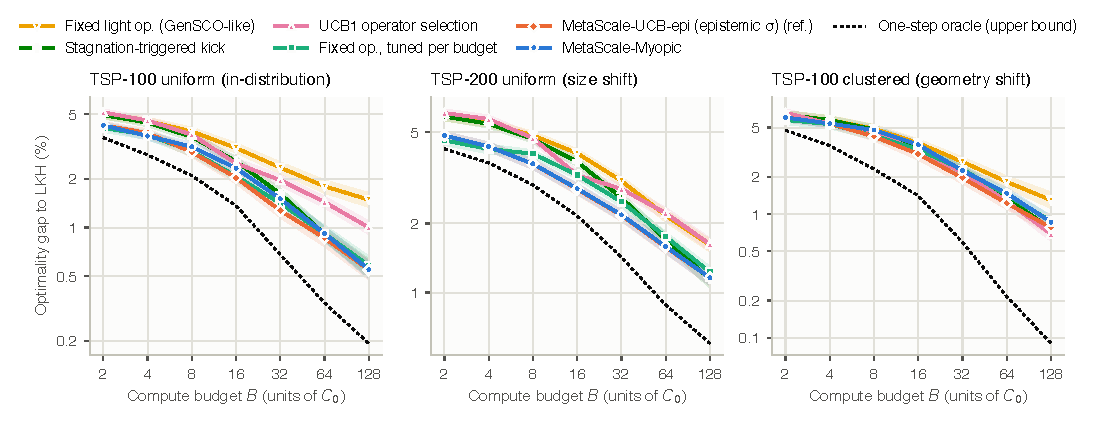
\includegraphics[width=0.86\textwidth]{figures/fig1_quality_compute_scaling.pdf}

		\vspace{-1mm}
		\raggedright\footnotesize
		Prototype của người trình bày (operator cổ điển thay GenSCO, TSP, 100 instance $\times$ 3 seed),
		\textbf{không phải kết quả của proposal}. Ref = MetaScale-UCB-epi. So với Fixed-light: tốt hơn 20/21 ô.
		So với Fixed-tuned: tốt hơn 8, kém 2, $\approx$ 11 ô (Wilcoxon signed-rank, Holm, $\alpha=0.05$); Friedman post-hoc $p_{\mathrm{Holm}}=0.24$.
	\end{frame}

	% ---------- S23 ----------
	\begin{frame}{Bài học từ prototype: cơ chế cần sửa trước khi lên GenSCO}
		\small
		\begin{tabular}{@{}p{0.36\textwidth}p{0.58\textwidth}@{}}
			\toprule
			Thành phần & Kết quả (21 ô = 3 tập test $\times$ 7 budget) \\
			\midrule
			$\sigma$ epistemic (ensemble) & tốt hơn $\sigma$ aleatoric của Eq.\,27: 7 ô tốt hơn, 1 ô kém \\
			History trong state & bỏ đi thì kém hơn 12/21 ô, không thắng ô nào \\
			VoC on-policy & Spearman $\rho$ chỉ 0.19--0.26 (0.47 trên log held-out) \\
			Learned \textsc{Stop} & không tiết kiệm compute so với chạy với budget nhỏ hơn \\
			Batch (Eq.\,31) & kém chia đều ở 4/6 cấu hình \\
			Wall-clock & 198\,µs/bước vs.\ 20\,µs (Fixed-tuned): operator cổ điển quá rẻ \\
			\bottomrule
		\end{tabular}

		\vspace{1mm}
		\smallnote{Nguồn số liệu: \texttt{mso/experiments/metascale-co-proto/REPORT.md}.}
		\keymsg{Distribution shift của offline RL hiện rõ; cần giai đoạn 2 (GenSCO) mới kết luận được}
	\end{frame}

	% ---------- Kết luận ----------
	\section{Kết luận}
	\begin{frame}{Kết luận: ý tưởng rõ, nhưng còn phải thắng lịch cố định đã tune}
		\footnotesize
		\begin{columns}[T]
			\begin{column}{0.5\textwidth}
				\textbf{Proposal đề xuất}
				\begin{itemize}\setlength\itemsep{1pt}
					\item Đổi câu hỏi: từ “tính \emph{bao nhiêu}” sang “tính \emph{cái gì}, khi nào dừng”
					\item Meta-controller (VoC + UCB + \textsc{Stop}) đứng trên solver frozen
				\end{itemize}
				\textbf{Đóng góp kỳ vọng} (Sec.\,12)
				\begin{itemize}\setlength\itemsep{1pt}
					\item Formulation tuần tự có budget; VoC có độ bất định; điều khiển đa trục, solver-agnostic
				\end{itemize}
			\end{column}
			\begin{column}{0.48\textwidth}
				\textbf{Hiện trạng}
				\begin{itemize}\setlength\itemsep{1pt}
					\item Mới là proposal, \alert{chưa có kết quả thực nghiệm}
					\item Phép thử quyết định: thắng \textbf{fixed tốt nhất ở từng budget} (Sec.\,14.2)
				\end{itemize}
				\textbf{Prototype của chúng tôi} (operator cổ điển)
				\begin{itemize}\setlength\itemsep{1pt}
					\item Thắng lịch một operator; \textbf{ngang} lịch cố định đã tune
					\item Bước tiếp: $\sigma$ epistemic, dữ liệu on-policy, chạy GenSCO trên GPU lab
				\end{itemize}
			\end{column}
		\end{columns}
		\keymsg{Giá trị của MetaScale-CO phụ thuộc vào việc controller thắng được lịch cố định đã tune khi dùng GenSCO}
	\end{frame}

\end{document}
